\begin{figure}
    \centering
    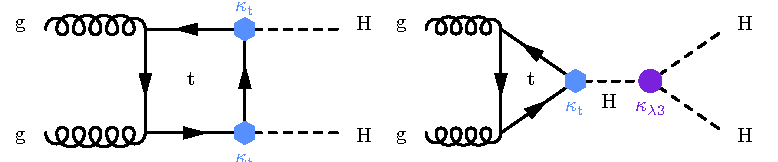
\includegraphics[width=\textwidth]{Diagrams/pdf/box_triag}\\[10pt]
    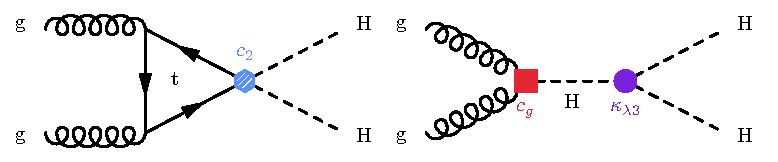
\includegraphics[width=\textwidth]{Diagrams/pdf/c2_cg}\\[10pt]
    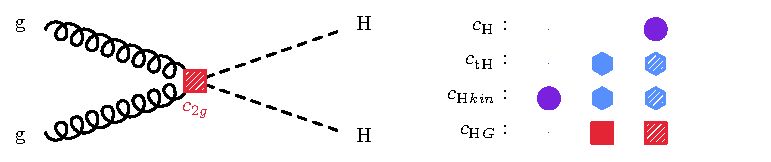
\includegraphics[width=\textwidth]{Diagrams/pdf/c_2g_smeft}
    \caption{Leading order Feynman diagrams contributing to \ggHH production. The markers indicate the HEFT couplings affecting each diagram, following the non-linear parameterization of Refs.~\cite{HEFT1,HHMatrix_R5}, and the panel on the right of the last row relates them to the leading dimension-6 SMEFT Wilson coefficients of Eq.~\eqref{eq:smeftL}~\cite{Buchalla:2018yce,Heinrich:2022huh}. The first row shows the diagrams that are also present in the SM, while the last two rows show the pure-BSM topologies that are unique to the EFT extensions.}
    \label{fig:feymnhh}
\end{figure}
